\section{Iteration 3: Decomposition of the Measurements Database Scheduler}
\label{add:it3}

\subsection{Step 1: Identify candidate drivers}
\label{add:it3/drivers}

\npar Remote measuring is the core business of the ReMeS system. Almost all
components in the ReMeS system need access to the measurements database.
However, not all queries on that database should be treated equally. For
instance, research queries have a lower priority than anomaly detection history
queries (see P3). Therefore, queries to the measurements database need to be
scheduled.

\npar The decomposition of this iteration is driven by

\begin{itemize}
	\item P3': Requests to the measurements database: These queries are subjected
	to a maximal execution time based on the SLA. 
\end{itemize}

\npar The functionality of two use cases is affected by this iteration. These
use cases are:

\begin{itemize}
  \item UC8': measurements have to be stored.
  \item UC17': researchers should be able to extract research data from the
  database (i.e. perform a read query).
\end{itemize}

\subsection{Step 2: Choose design concepts}
\label{add:it3/concepts}

\npar In this section there will be an overview of the chosen tactics and
patterns.

\subsubsection{Tactics}
\label{add:it3/tactics}

\npar The scheduler was introduced in iteration 1 (see section \ref{add:it1}) to
improve performance. At the level of the scheduler, performance is determined by
the scheduling policy. 

\npar The scheduling policy is defined by the quality attributes but the
scheduler itself can be implemented in different ways. One could use a single
queue for the scheduler. Jobs are pushed on a queue and popped off when the
scheduler can process a new job. 

\npar A scheduler can also be implemented with multiple queues. For each kind of
job, there is a separate queue. In this case, you would end up with a number of
queues for different priorities. Whenever a job resides in a queue for a long
time, it is promoted to a higher priority queue. 

\npar A scheduler must also guarantee that there will be no starvation among
jobs. Starvation happens when a job cannot execute because there always is a
job with a higher priority. When using a first in, first out policy, starvation
will not occur. However, when the database goes into overload mode, this might
become an issue. 

\npar To address this issue, a dynamic priority scheme will be used. The
priority of every job will be increased periodically. In this way, low priority
jobs will eventually have a high priority. 

\subsubsection{Design Patterns}
\label{add:it3/patterns}

\paragraph{Collections for States}

\npar The \emph{Collections for States} design pattern describes a way to
efficiently implement a scheduler with multiple queues. In a client, every state is
represented by a collection of objects with that state. The collections for
each state would be implemented with queues and the the states would represent
priority levels.

\paragraph{Strategy}

\npar If the scheduler allows for multiple policies, the \emph{Strategy} design
pattern can be used to implement these policies. The behaviour of the message router
will be determined by the policy.

\paragraph{Monitor} 

\npar Because the queues can be accessed by both the scheduler and the message
router, monitors have to be put in place to provide synchronization. This is
done to make sure that there aren't any concurrency issues within the scheduler. 

\paragraph{PriorityQueue}

\npar This is not a design pattern but a data type. This queue allows elements
to be inserted with a given priority. This could simplify the design by merging
all queues into one big queue.

\npar There is not really an advantage in having multiple queues. There is only
one instance that can process the jobs. The overhead of comparing the top
entries of the queues might also be large, making this solution less efficient. 

\subsection{Step 3: Instantiate architectural elements and allocate responsibilities}
\label{add:it3/elements}

\npar The decomposition of this component is shown in figure
\ref{fig:it3/elements}. 

\begin{figure}[H]
	\begin{centering}
		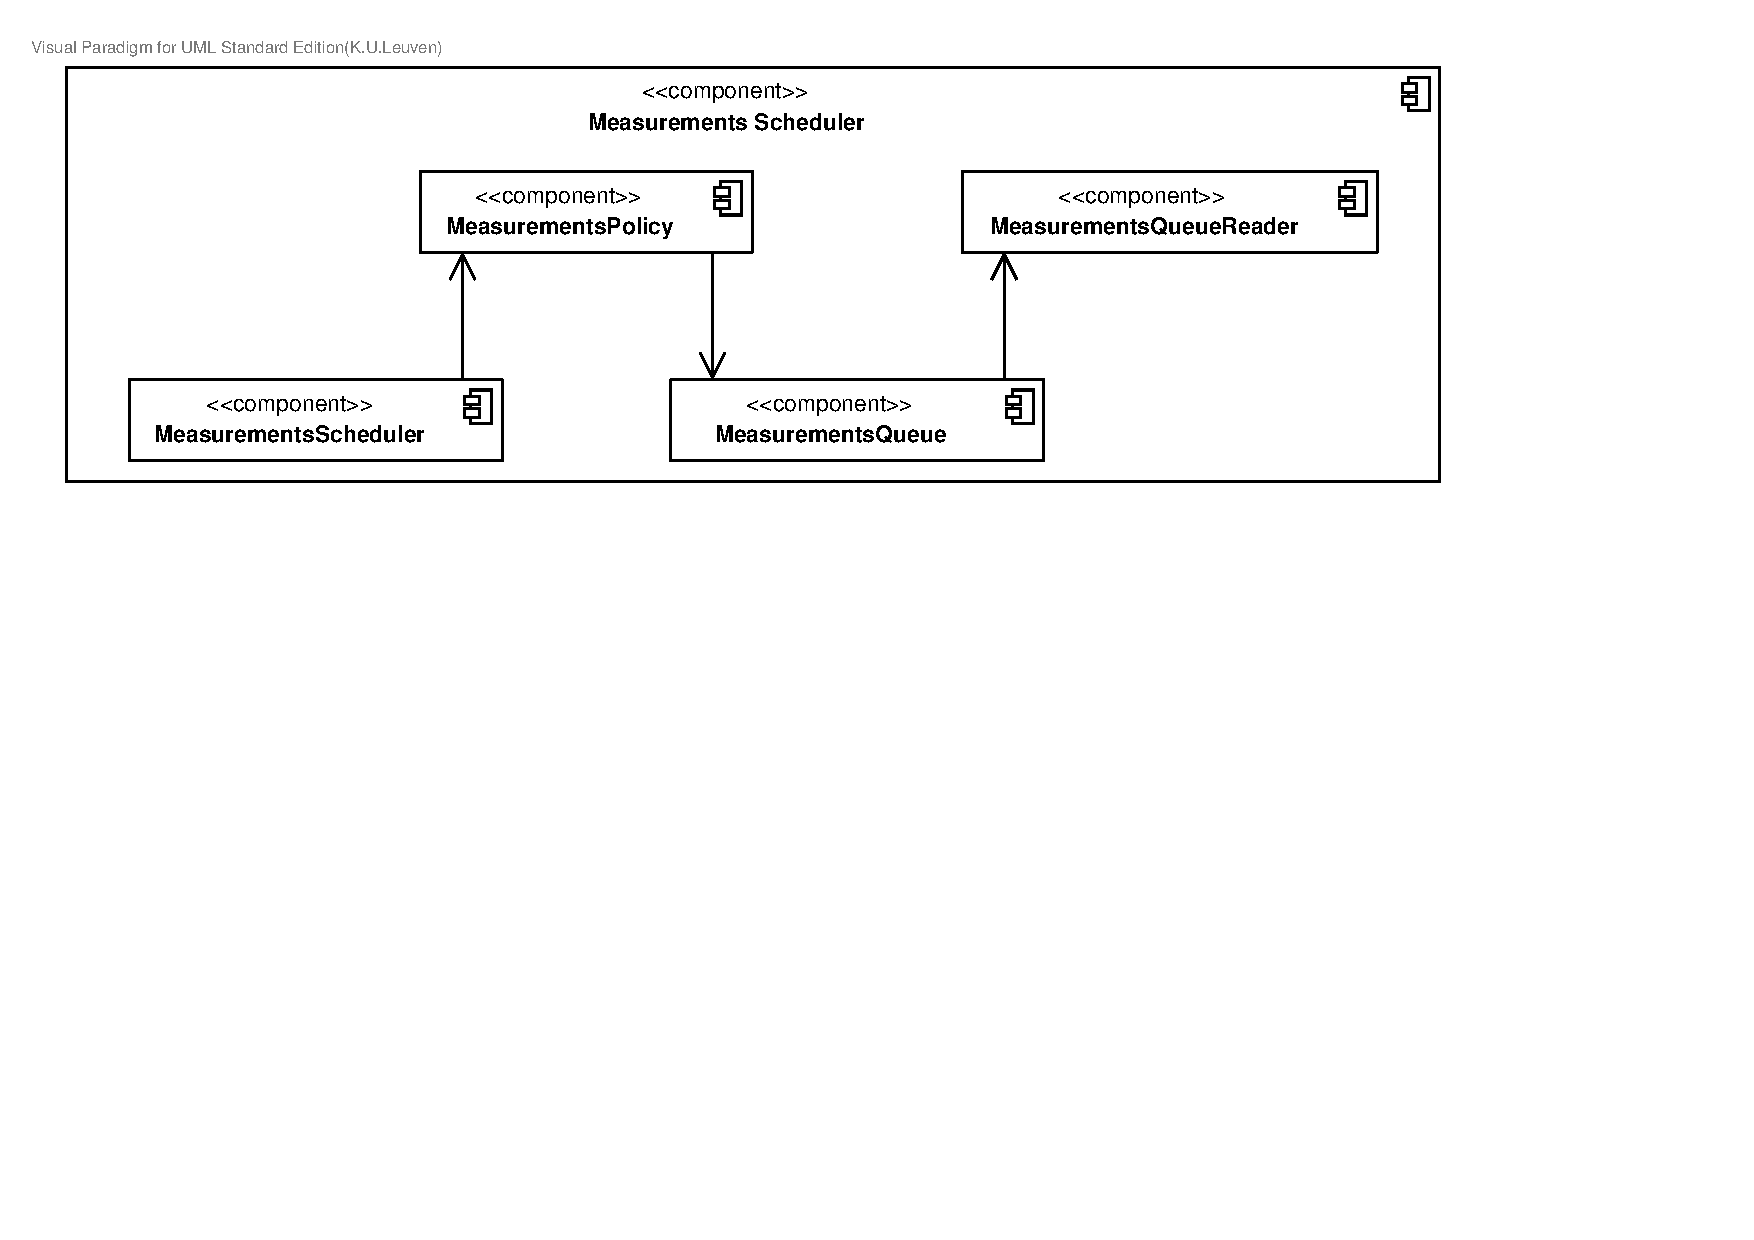
\includegraphics[width=\textwidth]{figs/add-it3-elements.pdf}
		\caption{Overview of the instantiated child components in the Scheduler For
		MeasurementsStorage.}
		\label{fig:it3/elements}
	\end{centering}
\end{figure}

\subsubsection{MeasurementsScheduler}

\npar The MeasurementsScheduler serves as entry point for the measurements
scheduling. Upon receiving a measurement the scheduler will place that
measurement in a MeasurementsPolicy. When the system transitions between load
modi (from normal to overload or vice versa) it is possible that another policy
is used. This transition in policies is likewise the responsibility of this
component.

\subsubsection{MeasurementsPolicy}

\npar A MeasurementsPolicy is responsible for inserting incoming
measurementsqueries (received from the MeasurementsScheduler) into the
MeasurementsQueue. To be able to do this, the policy first has to determine the
priority of the incoming query (and this priority is different for the various
policies).

\subsubsection{MeasurementsQueue}

\npar The MeasurementsQueue does nothing else than provide a priority queue for
measurementscommands with accompanying insert and retrieve functionality. Since
it is a priority queue the queries can be placed in different places in the
queue depending on their priority. More precisely, for each priority level will
the index of the last element with that priority be kept in a list. When a new
query needs to be inserted, the priority of that query is determined.
Subsequently, the priority is used to retrieve the index of the last element and
in this way the new query can be inserted. The priorities of all commands are
increased every time a new command is inserted to prevent starvation.

\subsubsection{MeasurementsQueueReader}

\npar The purpose of this component is dequeueing the MeasurementsQueue and
afterwards dispatch the popped query to the the MeasurementsStorage.

% \npar All requests to the Measurements Database Scheduler are encapsulated as
% QueryCommand objects. These objects have already been created in another
% component and represent a query to the measurements database. Because the
% scheduling makes communication asynchronous, the QueryCommand contains a
% Callback to return the result of the query to the issuer.
% 
% \npar The scheduler (MeasurementsScheduler) handles every incoming command
% (QueryCommand) by inserting the command in a queue (MeasurementsQueue) with a
% certain priority using a policy (MeasurementsPolicy). The scheduling policy
% determines the priority of the command based on the nature of that command. 
% 
% \npar An additional component (MeasurementsQueueReader) will pop the command
% with the highest priority off the queue and present it on the database for execution. 

\subsection{Step 4: Define interfaces for instantiated elements}
\label{add:it3/interfaces}

\npar In this section each interface is explained in terms of the components
which use and/or offer it together with information about what is exchanged. For
detailed information with reference to the specific methods the interfaces
implement, we refer to the interface catalog, see appendix
\ref{chap:interface-catalog}.

\subsubsection{MeasurementsSchedulerAPI}

\npar This interface was already discussed in iteration 1, see
\ref{add:it1/interfaces}.

\subsubsection{MeasurementsPolicyAPI}

\npar The \interface{MeasurementsPolicyAPI} lies between the
MeasurementsScheduler and the MeasurementsPolicy. Its goal is to pass through
commands which have to be placed in a MeasurementQueue.

\subsubsection{MeasurementsQueueAPI}

\npar This interface is offered by the MeasurementsQueue and used by both the
MeasurementsPolicy and the MeasurementsQueueReader. The policy uses the
interface to place commands in the queue and the reader pops them off.

\npar Figure \ref{fig:it3/interfaces} summarizes the components and the
interfaces instantiated in this iteration.

\begin{figure}[H]
	\begin{centering}
		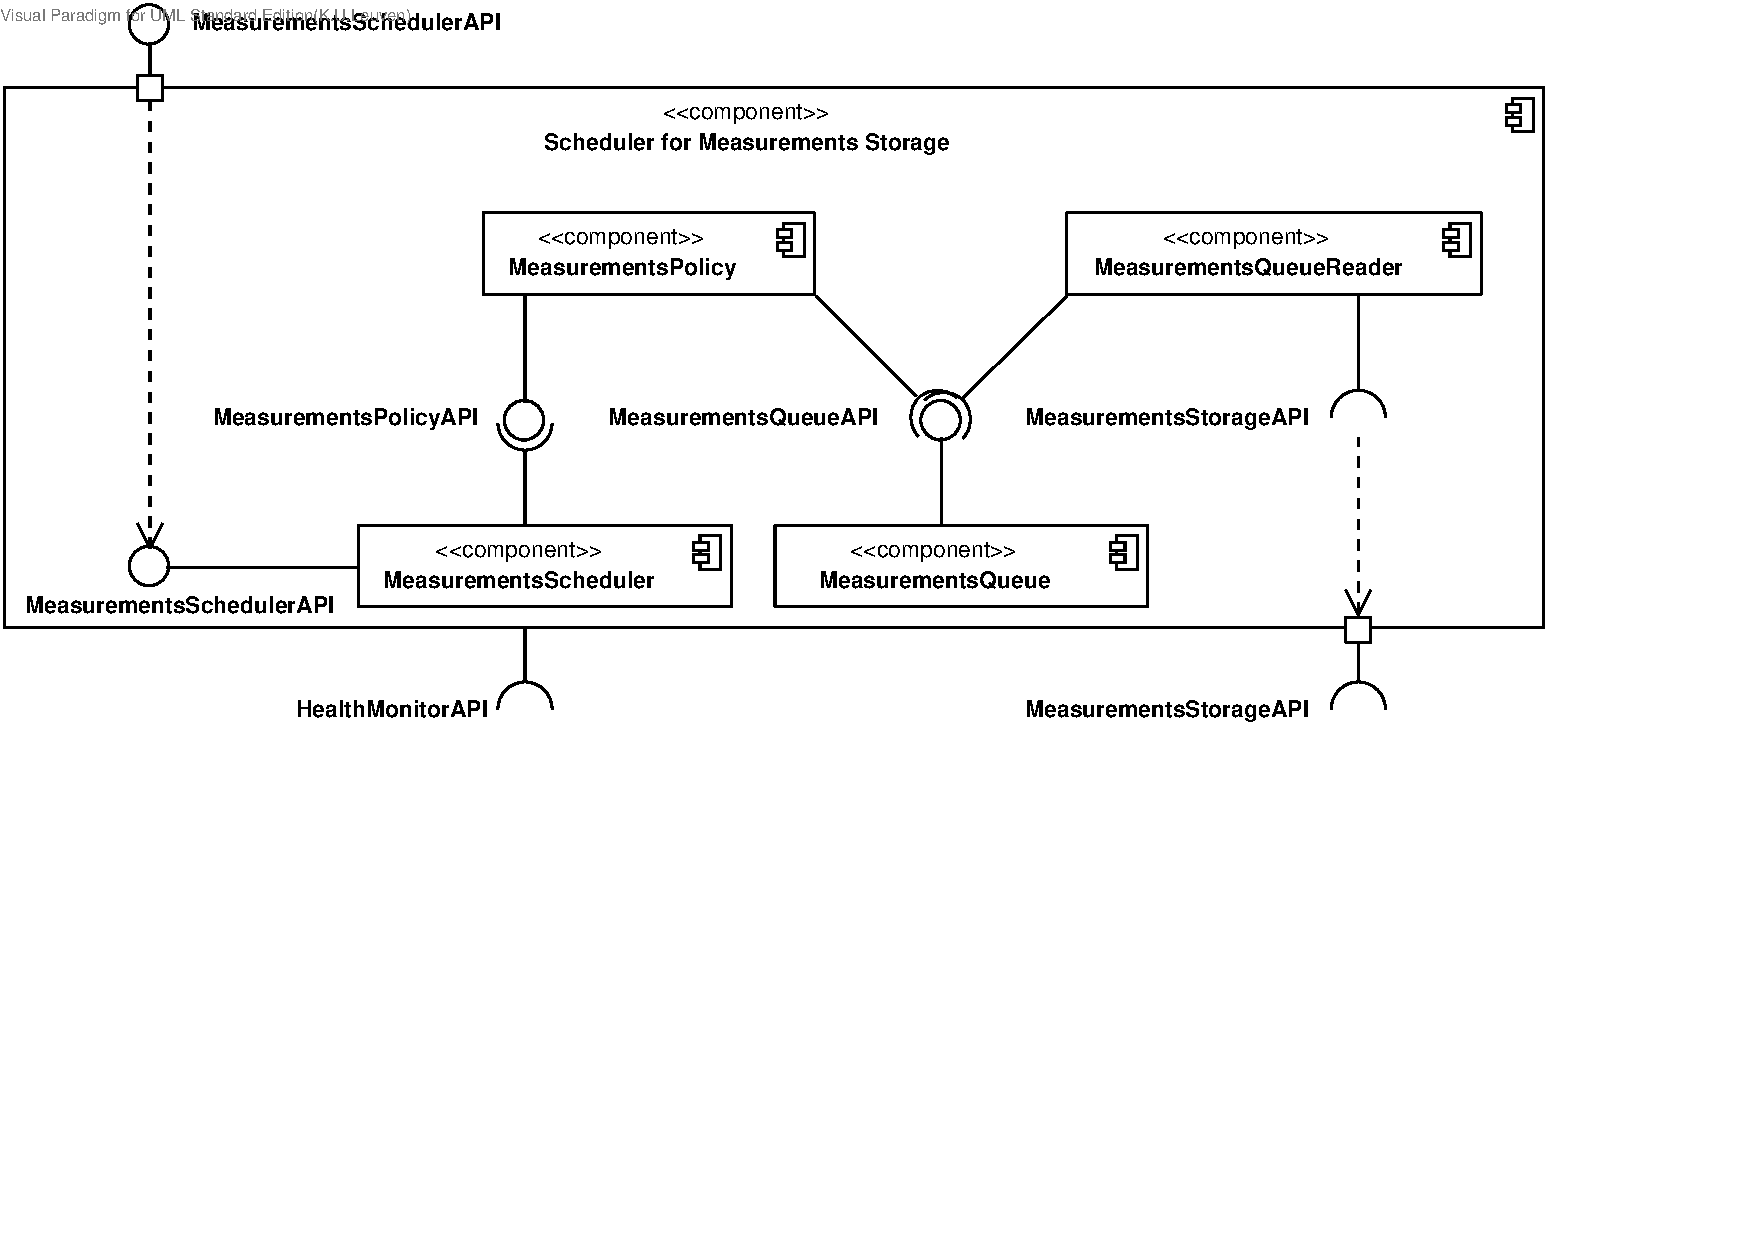
\includegraphics[width=\textwidth]{figs/add-it3-interfaces.pdf}
		\caption{Overview of the interfaces and components in the Scheduler For
		MeasurementsStorage.}
		\label{fig:it3/interfaces}
	\end{centering}
\end{figure}

\subsection{Step 5: Verify and refine}
\label{add:it3/verification}

\npar The one and only driver for this iteration, P3', is resolved. The
scheduler and scheduling policy guarantee that QueryCommands are executed in the
right order.